\documentclass[tikz,border=6pt]{standalone}
\usepackage{amsmath,amssymb}
\usetikzlibrary{arrows.meta,positioning,calc,fit,decorations.pathreplacing}

\begin{document}
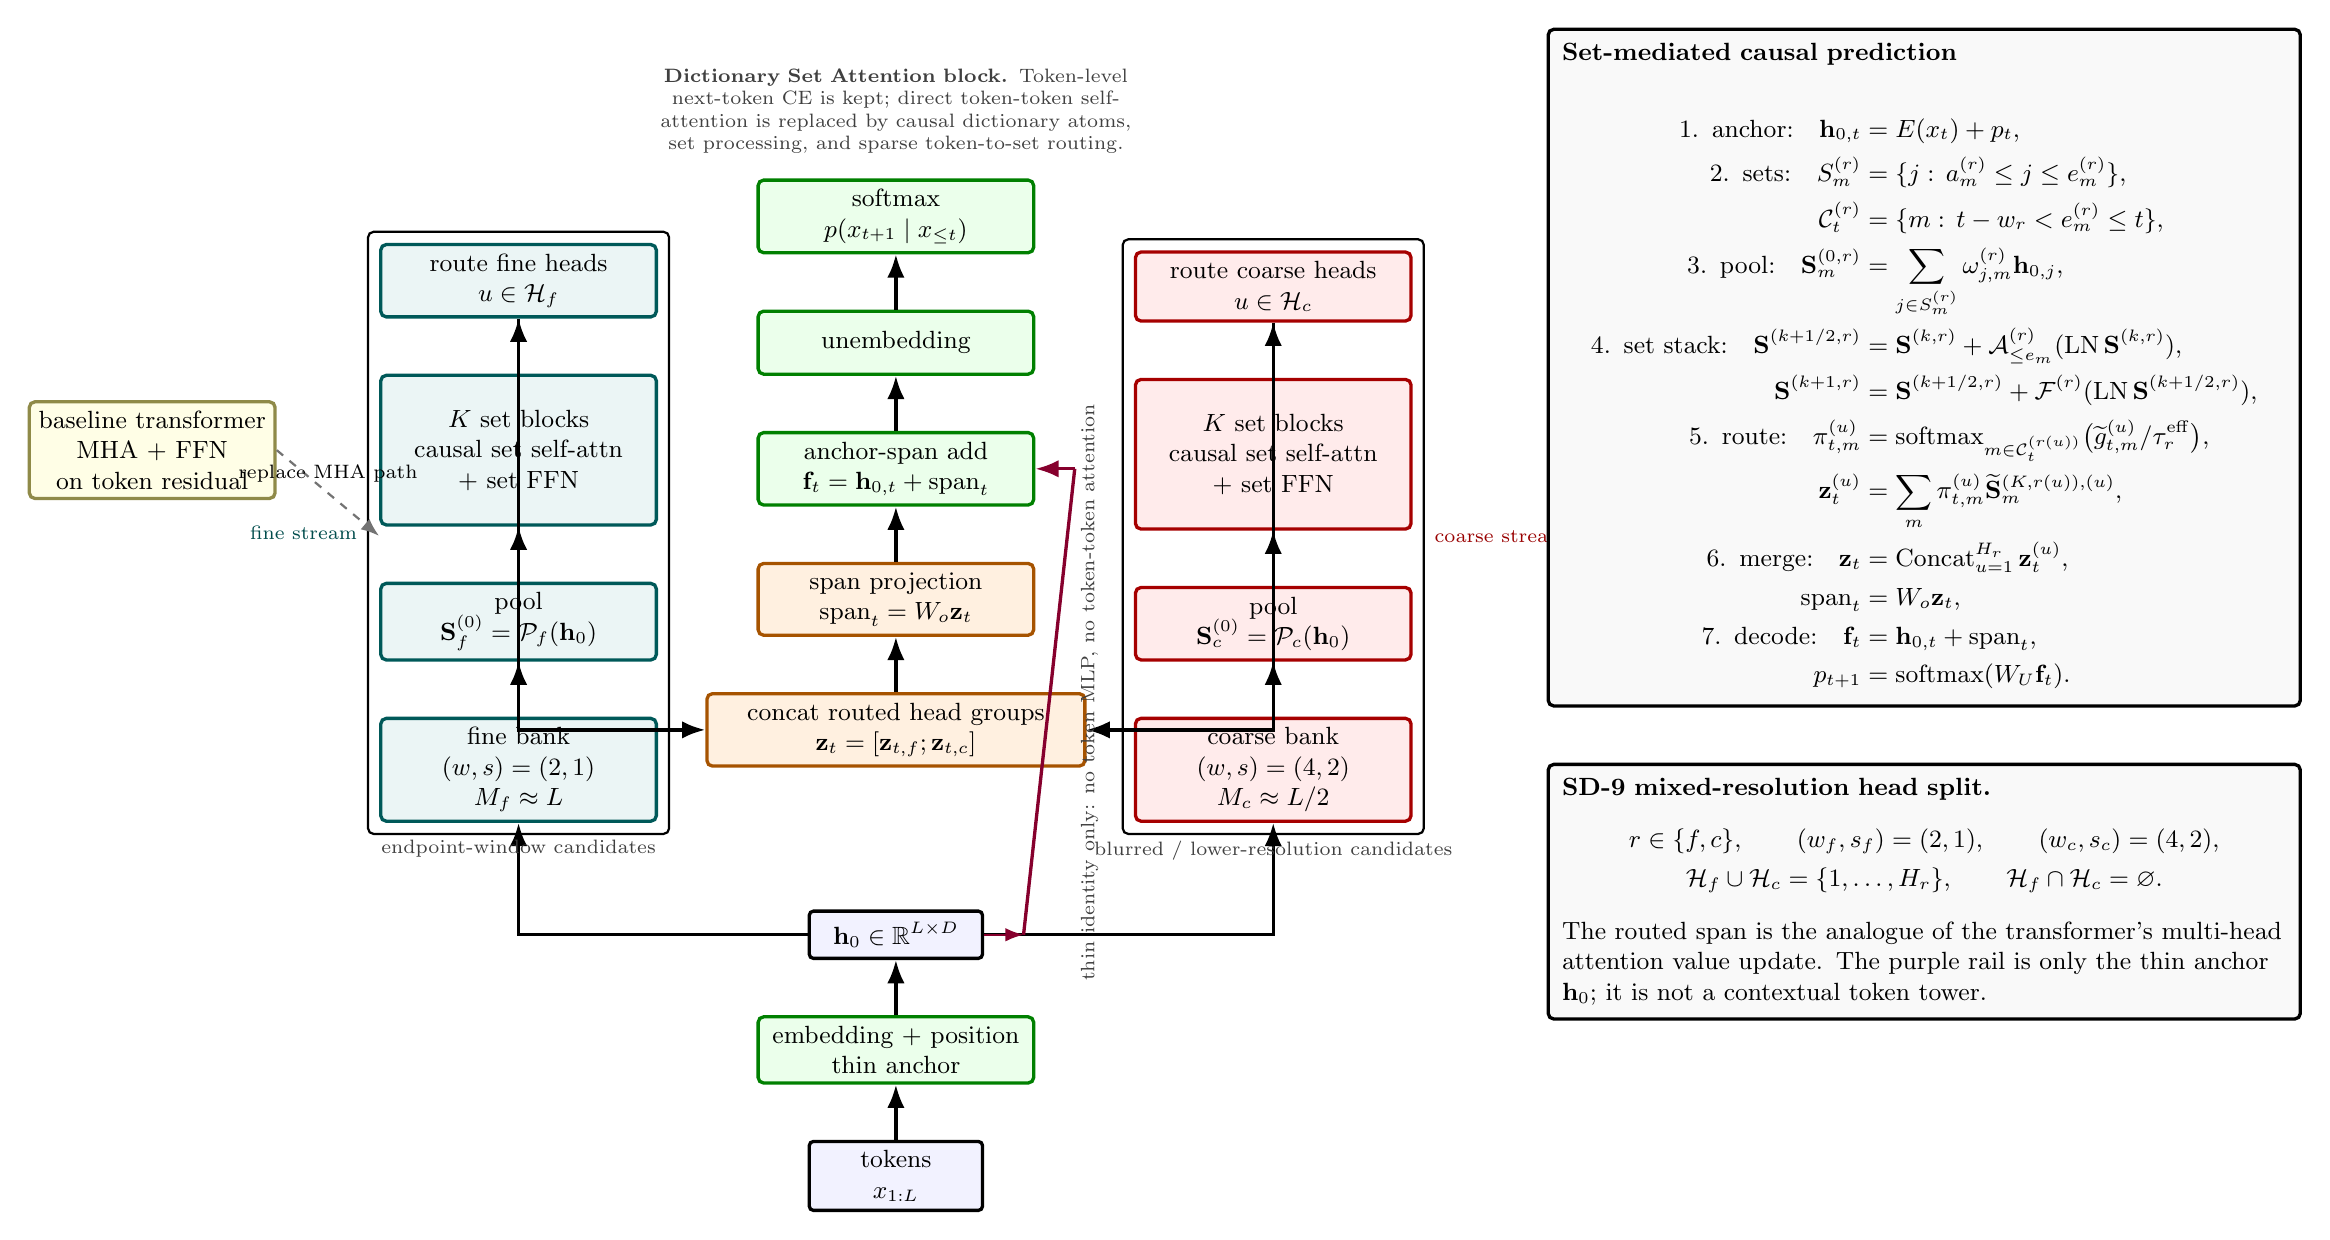
\begin{tikzpicture}[
  font=\small,
  >=Latex,
  node distance=7mm,
  block/.style={draw, rounded corners=2pt, very thick, align=center,
    minimum width=35mm, minimum height=8mm, fill=white},
  op/.style={block, fill=green!8, draw=green!50!black},
  setop/.style={block, fill=cyan!8, draw=cyan!55!black},
  routeop/.style={block, fill=orange!12, draw=orange!65!black},
  mathbox/.style={draw, rounded corners=2pt, very thick, align=left,
    fill=gray!5, inner sep=5pt, text width=92mm},
  tensor/.style={draw, rounded corners=1.5pt, very thick, fill=blue!5,
    minimum width=22mm, minimum height=6mm, align=center},
  note/.style={align=center, font=\scriptsize, text=black!75},
  arr/.style={->, very thick},
  thinarr/.style={->, thick},
  skip/.style={->, very thick, draw=purple!70!black},
  residual/.style={very thick, draw=purple!70!black},
  fine/.style={draw=teal!70!black, fill=teal!8},
  coarse/.style={draw=red!65!black, fill=red!8}
]

% Left: architecture.
\node[tensor] (tok) {tokens\\$x_{1:L}$};
\node[op, above=of tok] (embed) {embedding + position\\thin anchor};
\node[tensor, above=of embed] (h0) {$\mathbf h_0\in\mathbb R^{L\times D}$};

\node[setop, above left=11mm and 19mm of h0, fine] (finebank)
  {fine bank\\$(w,s)=(2,1)$\\$M_f\approx L$};
\node[setop, above right=11mm and 19mm of h0, coarse] (coarsebank)
  {coarse bank\\$(w,s)=(4,2)$\\$M_c\approx L/2$};
\node[setop, above=of finebank, fine] (finepool)
  {pool\\$\mathbf S_f^{(0)}=\mathcal P_f(\mathbf h_0)$};
\node[setop, above=of coarsebank, coarse] (coarsepool)
  {pool\\$\mathbf S_c^{(0)}=\mathcal P_c(\mathbf h_0)$};
\node[setop, above=of finepool, minimum height=19mm, fine] (finestack)
  {$K$ set blocks\\causal set self-attn\\+ set FFN};
\node[setop, above=of coarsepool, minimum height=19mm, coarse] (coarsestack)
  {$K$ set blocks\\causal set self-attn\\+ set FFN};
\node[routeop, above=of finestack, fine] (fineroute)
  {route fine heads\\$u\in\mathcal H_f$};
\node[routeop, above=of coarsestack, coarse] (coarseroute)
  {route coarse heads\\$u\in\mathcal H_c$};

\node[routeop, above=18mm of h0, xshift=0mm, minimum width=48mm] (concat)
  {concat routed head groups\\$\mathbf z_t=[\mathbf z_{t,f};\mathbf z_{t,c}]$};
\node[routeop, above=of concat] (proj)
  {span projection\\$\mathrm{span}_t=W_o\mathbf z_t$};
\node[op, above=of proj] (add)
  {anchor-span add\\$\mathbf f_t=\mathbf h_{0,t}+\mathrm{span}_t$};
\node[op, above=of add] (unembed) {unembedding};
\node[op, above=of unembed] (softmax) {softmax\\$p(x_{t+1}\mid x_{\le t})$};

\draw[arr] (tok) -- (embed);
\draw[arr] (embed) -- (h0);
\draw[arr] (h0) -| (finebank);
\draw[arr] (h0) -| (coarsebank);
\draw[arr] (finebank) -- (finepool);
\draw[arr] (coarsebank) -- (coarsepool);
\draw[arr] (finepool) -- (finestack);
\draw[arr] (coarsepool) -- (coarsestack);
\draw[arr] (finestack) -- (fineroute);
\draw[arr] (coarsestack) -- (coarseroute);
\draw[arr] (fineroute) |- (concat);
\draw[arr] (coarseroute) |- (concat);
\draw[arr] (concat) -- (proj);
\draw[arr] (proj) -- (add);
\draw[arr] (add) -- (unembed);
\draw[arr] (unembed) -- (softmax);

% Thin identity residual rail.
\draw[residual] ($(h0.east)+(5mm,0)$) -- ($(add.east)+(5mm,0)$);
\draw[thinarr, draw=purple!70!black] (h0.east) -- ($(h0.east)+(5mm,0)$);
\draw[skip] ($(add.east)+(5mm,0)$) -- (add.east);
\node[note, rotate=90] at ($(h0.east)!0.52!(add.east)+(10mm,0)$)
  {thin identity only: no token MLP, no token-token attention};

\node[note, below=1mm of finebank] {endpoint-window candidates};
\node[note, below=1mm of coarsebank] {blurred / lower-resolution candidates};

\node[draw, rounded corners=2pt, thick, fit=(finebank)(finepool)(finestack)(fineroute),
  inner sep=4pt, label={[font=\scriptsize, text=teal!60!black]left:fine stream}] {};
\node[draw, rounded corners=2pt, thick, fit=(coarsebank)(coarsepool)(coarsestack)(coarseroute),
  inner sep=4pt, label={[font=\scriptsize, text=red!60!black]right:coarse stream}] {};

% Right: aligned math.
\node[mathbox, right=17mm of coarsestack, yshift=11mm] (eqs) {
\textbf{Set-mediated causal prediction}\\[-1mm]
\begin{align*}
\text{1. anchor:}\quad
  \mathbf h_{0,t} &= E(x_t)+p_t,\\
\text{2. sets:}\quad
  S^{(r)}_m &= \{j:\, a^{(r)}_m\le j\le e^{(r)}_m\},\\
  \mathcal C^{(r)}_t
    &= \{m:\, t-w_r<e^{(r)}_m\le t\},\\
\text{3. pool:}\quad
  \mathbf S^{(0,r)}_m
    &= \sum_{j\in S^{(r)}_m}\omega^{(r)}_{j,m}\mathbf h_{0,j},\\
\text{4. set stack:}\quad
  \mathbf S^{(k+1/2,r)}
    &= \mathbf S^{(k,r)}
     + \mathcal A^{(r)}_{\le e_m}(\operatorname{LN}\mathbf S^{(k,r)}),\\
  \mathbf S^{(k+1,r)}
    &= \mathbf S^{(k+1/2,r)}
     + \mathcal F^{(r)}(\operatorname{LN}\mathbf S^{(k+1/2,r)}),\\
\text{5. route:}\quad
  \pi_{t,m}^{(u)}
    &= \operatorname{softmax}_{m\in\mathcal C^{(r(u))}_t}
       \bigl(\widetilde g_{t,m}^{(u)}/\tau_r^{\mathrm{eff}}\bigr),\\
  \mathbf z_t^{(u)}
    &= \sum_m \pi_{t,m}^{(u)}
       \widetilde{\mathbf S}^{(K,r(u)),(u)}_m,\\
\text{6. merge:}\quad
  \mathbf z_t
    &= \operatorname{Concat}_{u=1}^{H_r}\mathbf z_t^{(u)},\\
  \mathrm{span}_t &= W_o\mathbf z_t,\\
\text{7. decode:}\quad
  \mathbf f_t &= \mathbf h_{0,t}+\mathrm{span}_t,\\
  p_{t+1} &= \operatorname{softmax}(W_U\mathbf f_t).
\end{align*}
};

\node[mathbox, below=7mm of eqs, text width=92mm] (legend) {
\textbf{SD-9 mixed-resolution head split.}
\[
\begin{gathered}
r\in\{f,c\},\qquad (w_f,s_f)=(2,1),\qquad (w_c,s_c)=(4,2),\\
\mathcal H_f\cup\mathcal H_c=\{1,\dots,H_r\},\qquad
\mathcal H_f\cap\mathcal H_c=\varnothing .
\end{gathered}
\]
The routed span is the analogue of the transformer's multi-head attention
value update.  The purple rail is only the thin anchor \(\mathbf h_0\); it is
not a contextual token tower.
};

\node[note, above=2mm of softmax, text width=70mm, align=center] (caption)
  {\textbf{Dictionary Set Attention block.} Token-level next-token CE is kept; direct token-token self-attention is replaced by causal dictionary atoms, set processing, and sparse token-to-set routing.};

% Dashed baseline cue.
\node[block, left=13mm of finestack, minimum width=28mm, fill=yellow!10, draw=yellow!50!black] (baseline)
  {baseline transformer\\MHA + FFN\\on token residual};
\draw[thinarr, dashed, draw=black!55] (baseline.east) -- node[above, font=\scriptsize]
  {replace MHA path} ($(finestack.west)!0.5!(finepool.west)$);

\end{tikzpicture}
\end{document}
